\documentclass{zhvt-classic}

\zhvtset{
    grid_lines = false,
    main_font           = KingHwa_OldSong,  % 字体
    % font_size           = 27.32pt,  % 字体尺寸,三分,9.6mm,直接用 9.6mm 会有奇怪的问题
    % baselineskip_ratio  = 1.5,  % 行距与字体尺寸的倍数
    jiazhu_font         = KingHwa_OldSong,  % 夹注字体
    title_font          = KingHwa_OldSong,  % 书名标题字体
}

\title{畫譜}
\ExplSyntaxOn
\mark_insert:nn { zhvt_chapter } { 山水卷九 }
\ExplSyntaxOff
\begin{document}
~\vspace{5pt}\par
\hfil 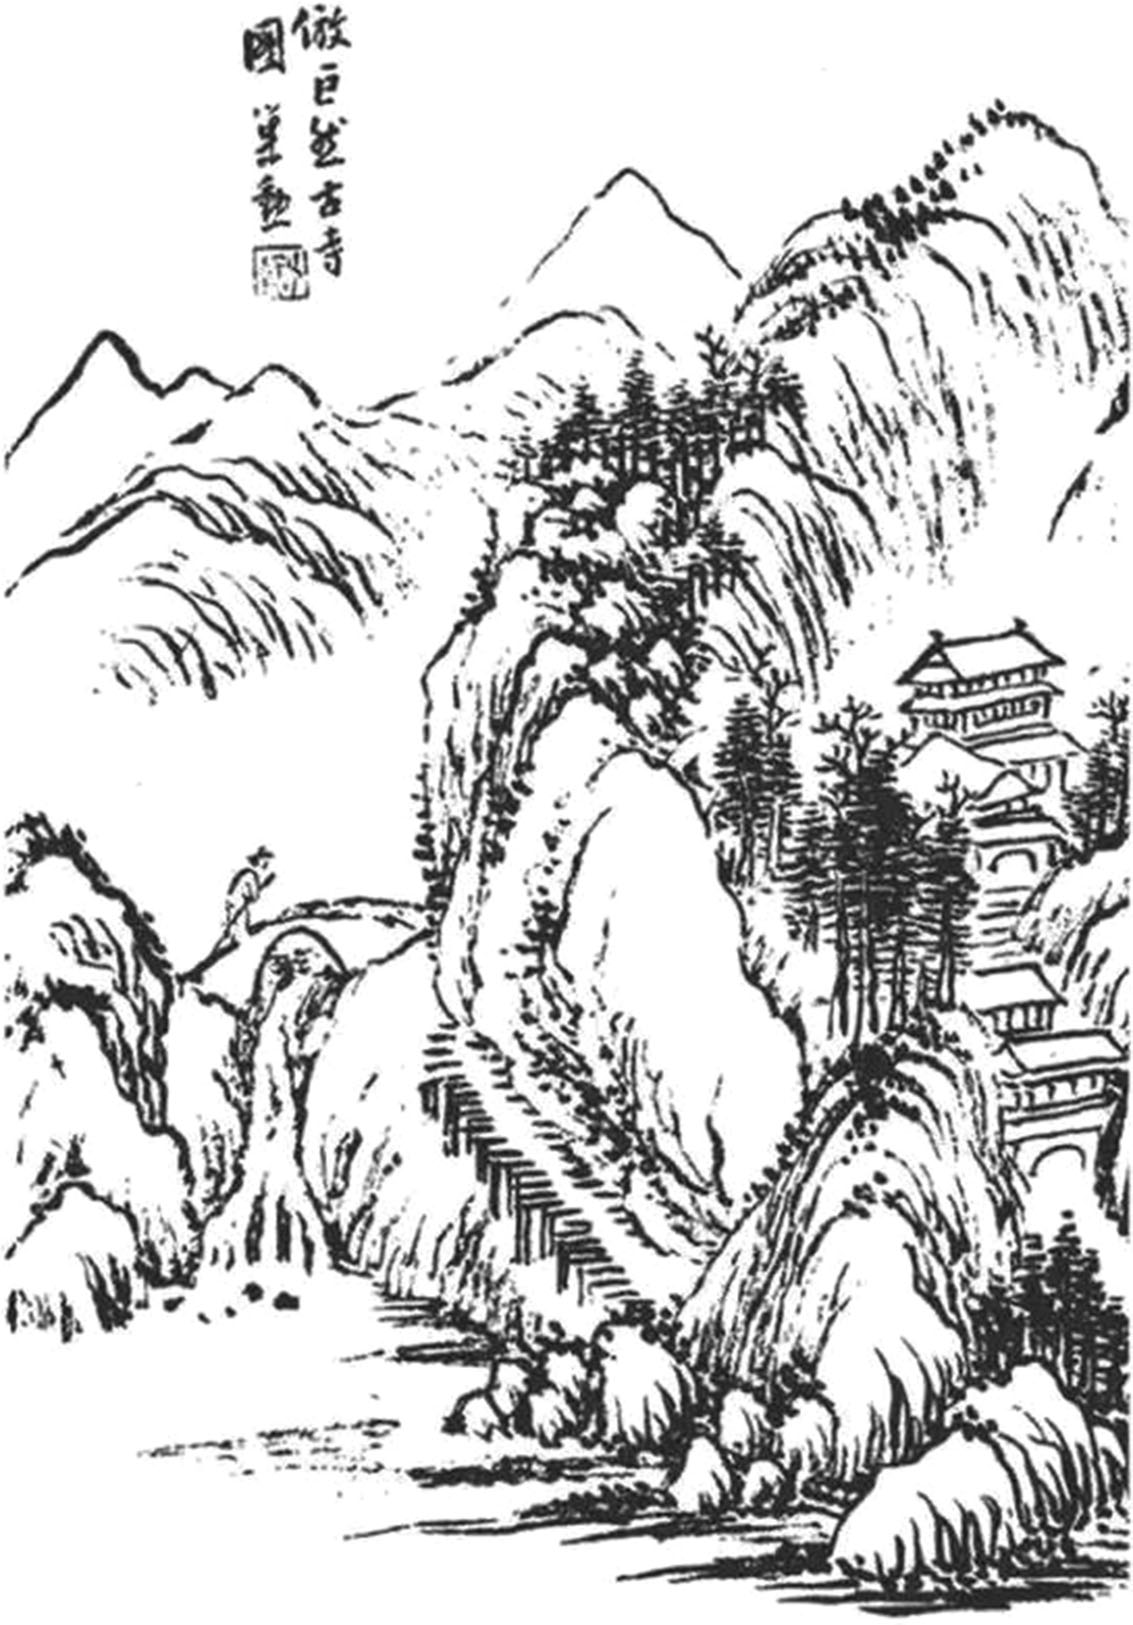
\includegraphics[angle=90]{paint01}
\clearpage
~\vspace{5pt}\par
\hfil 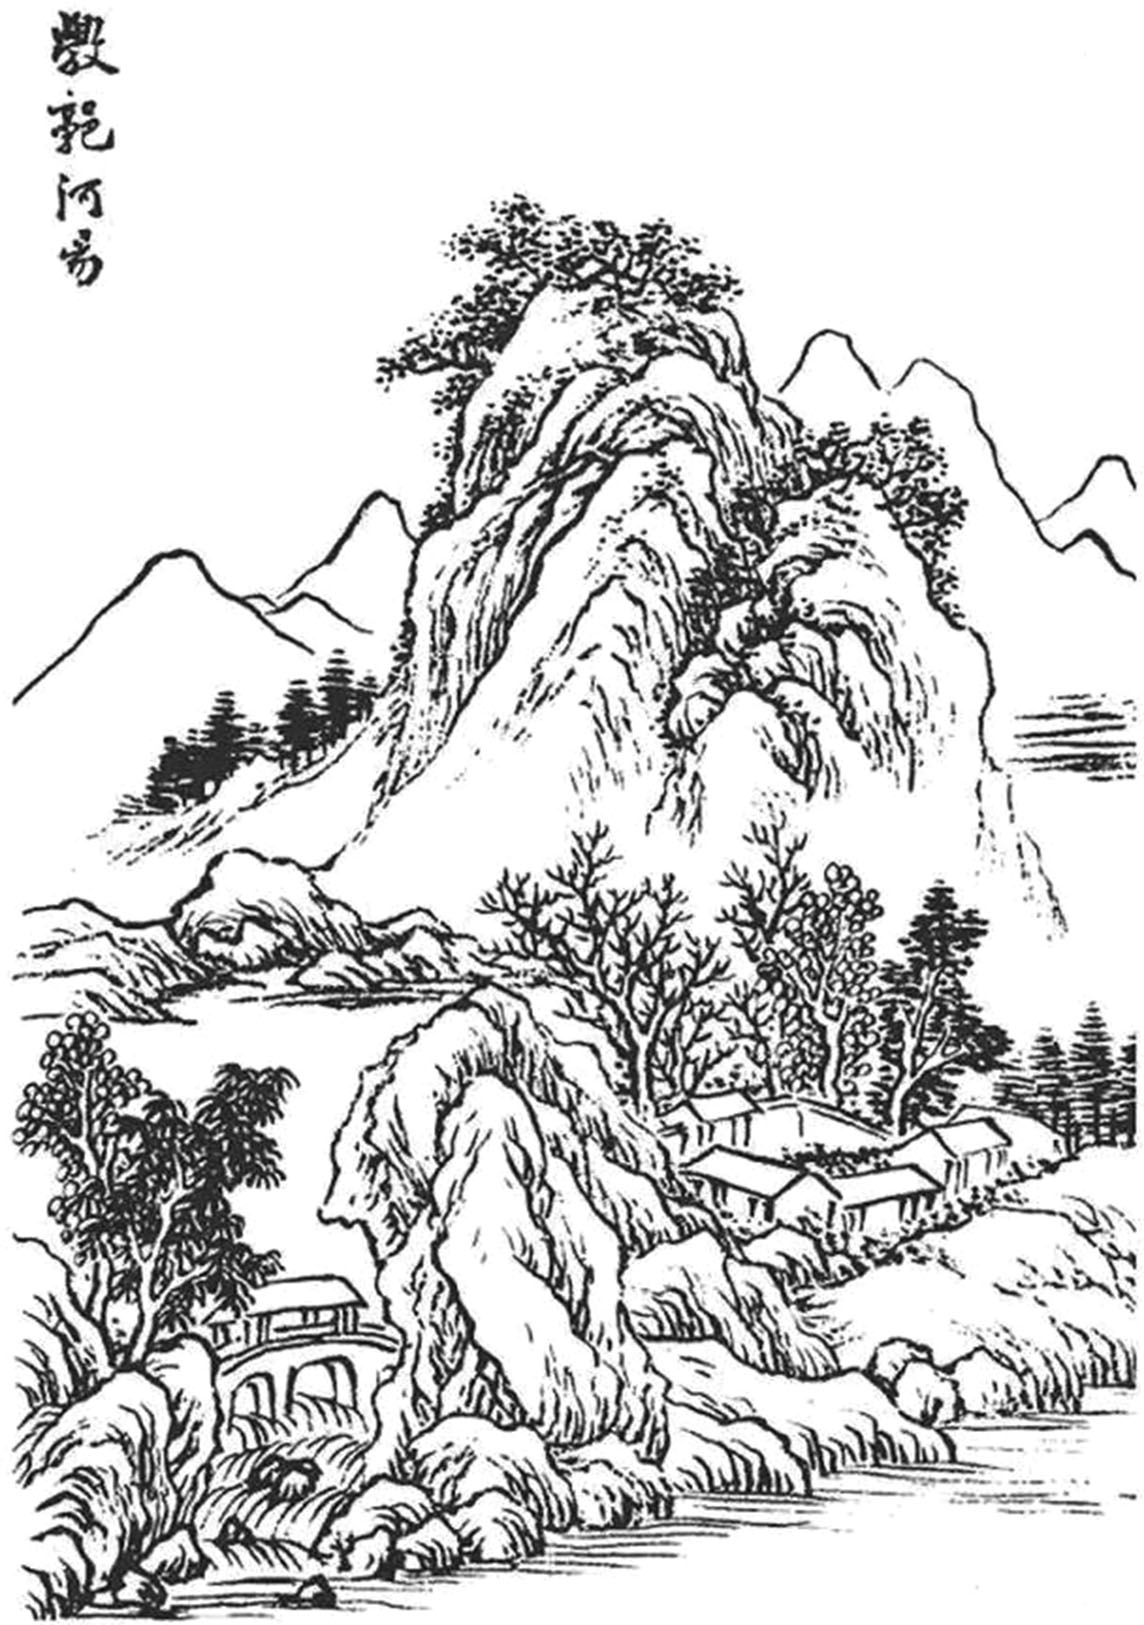
\includegraphics[angle=90]{paint02}
\clearpage
\end{document}